\documentclass[11pt, letterpaper]{article}

\usepackage[margin=1in]{geometry}
\usepackage{graphicx}

% Resolve image references whether the build runs from LEAI/docs/ (the
% intended cwd) or from the repository root (e.g. when latexmk is fired
% by an editor task from the project root). Listing both prefixes makes
% \includegraphics{screenshots/foo.png} resolve in either case.
\graphicspath{{./}{LEAI/docs/}}

\usepackage{hyperref}
\usepackage{xcolor}
\usepackage{booktabs}
\usepackage{enumitem}
\usepackage{fancyvrb}
\usepackage{fvextra}  % gives Verbatim the breaklines / breaksymbol options
\usepackage{tcolorbox}
\usepackage{titlesec}
\usepackage{parskip}
\usepackage{placeins}  % \FloatBarrier — keep figures inside their section
\usepackage{float}     % [H] placement specifier — pin a figure to its text
\usepackage[hypcap=true]{caption}  % anchor hyperref links at top of figure, not caption

% Colors
\definecolor{linkblue}{HTML}{2563EB}
\definecolor{urgentred}{HTML}{DC2626}
\definecolor{urgentamber}{HTML}{D97706}
\definecolor{urgentgreen}{HTML}{16A34A}
\definecolor{tipbg}{HTML}{F0F9FF}
\definecolor{tipborder}{HTML}{3B82F6}

\hypersetup{
    colorlinks=true,
    linkcolor=linkblue,
    urlcolor=linkblue,
}

\titleformat{\section}{\Large\bfseries}{}{0em}{}[\vspace{-0.5em}\rule{\textwidth}{0.4pt}]
\titleformat{\subsection}{\large\bfseries}{}{0em}{}

% Tip box
\newtcolorbox{tipbox}{
    colback=tipbg,
    colframe=tipborder,
    boxrule=0.5pt,
    arc=2pt,
    left=8pt, right=8pt, top=6pt, bottom=6pt,
}

\begin{document}

\begin{center}
    {\LARGE\bfseries LEAI Instructor Guide}\\[0.5em]
    {\large Learning Experience AI}\\[1em]
    {\normalsize GUII Lab — UC Santa Cruz}
\end{center}

\vspace{1em}

\textbf{Learning Experience AI (LEAI)} is a course feedback infrastructure for CM instructors. It replaces end-of-quarter surveys with conversational, mid-course check-ins that you can deploy as often as you need --- and gives you AI-generated summaries of what your students are actually experiencing.

\section{How It Works --- 3-Minute Overview}

\begin{center}
\begin{tabular}{ccccc}
\textbf{You (Prompt Designer)} & $\rightarrow$ & \textbf{Students (FeedbackCollector)} & $\rightarrow$ & \textbf{You (Feedback Analyzer)} \\
Configure a survey & & Chat with the AI & & See themes + insights \\
Get a shareable link & & \textasciitilde5--10 min per student & & \\
\end{tabular}
\end{center}

Each ``survey'' is a short AI-facilitated conversation. Students follow a link, talk to the AI about the course, and you see aggregated themes and friction points --- without reading 40 individual responses.

\section{Part 1: Prompt Designer}

\textbf{URL:} \url{https://guiilab.github.io/LEAI/PromptDesigner.html}

This is where you set up your course and create surveys. You do this once per course, then return each week to create a new survey.

\subsection{Step 1 --- Create Your Course}

Fill in four fields:

\begin{table}[h!]
\centering
\begin{tabular}{@{}llp{7cm}@{}}
\toprule
\textbf{Field} & \textbf{Example} & \textbf{Notes} \\
\midrule
Course ID & \texttt{cm115-sp26} & Lowercase, hyphens only. Appears in all your survey links. \\
Course Name & \texttt{Game Design \& Interactive Media} & Shown in the dashboard header. \\
Your Name & \texttt{Prof.\ Alex Chen} & Stored with the course config. \\
Dashboard Password & \texttt{feedback2026} & Protects your analytics dashboard. Share only with co-instructors or TAs. \\
\bottomrule
\end{tabular}
\end{table}

Click \textbf{Create Course}.

\begin{tipbox}
If you're returning to a course you already set up, scroll down to \textbf{``Already have a course?''}, enter your Course ID and password, and click \textbf{Unlock Course}.
\end{tipbox}

\begin{figure}[h!]
\centering
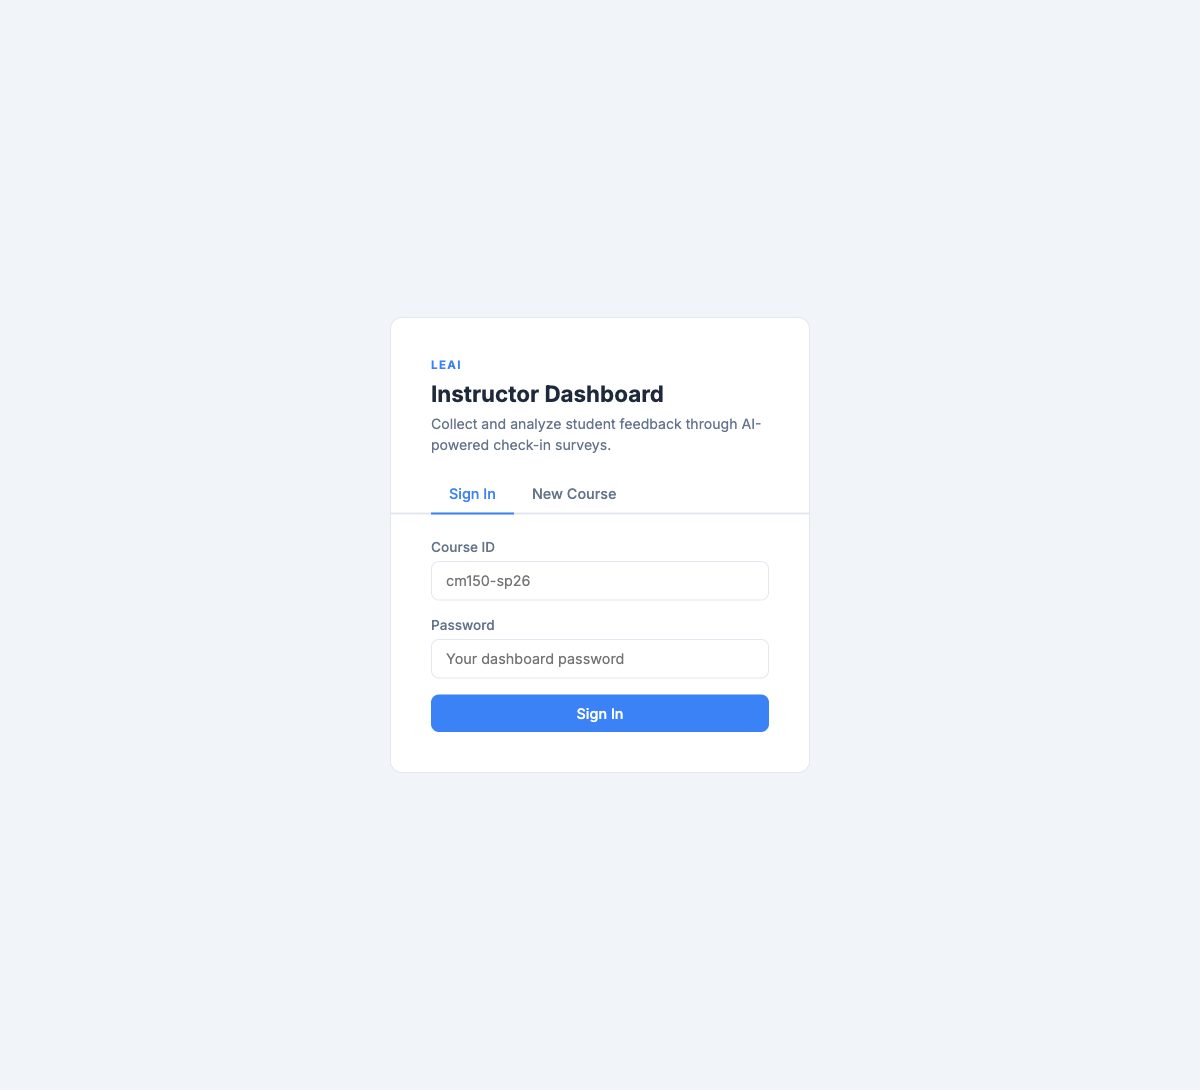
\includegraphics[width=\textwidth]{screenshots/01-prompt-designer-setup.png}
\caption{Prompt Designer --- Course Setup}
\end{figure}

\subsection{Step 2 --- Create a Survey}

Once your course is active, the \textbf{New Survey} form appears on the left:

\begin{table}[h!]
\centering
\begin{tabular}{@{}llp{7cm}@{}}
\toprule
\textbf{Field} & \textbf{Example} & \textbf{Notes} \\
\midrule
Week / Milestone & \texttt{6} & Used to order surveys in your dashboard. \\
Survey Label & \texttt{Week 6 --- Team Dynamics Check-in} & Shown to students as the page title. Keep it brief. \\
System Prompt & \emph{(see below)} & Instructions that shape how the AI conducts the conversation. \\
\bottomrule
\end{tabular}
\end{table}

\textbf{Writing a good system prompt} is the most important step. It defines what the AI asks about and how it follows up. A few principles:

\begin{itemize}[nosep]
    \item Be specific about the topic (e.g., ``team collaboration,'' ``assignment clarity,'' ``prototype experience'')
    \item Tell it the tone --- ``warm and conversational,'' ``keep it short,'' ``probe gently''
    \item Mention the course context so the AI doesn't ask generic questions
\end{itemize}

\textbf{Example prompt for a week 6 team check-in:}

\begin{Verbatim}[fontsize=\small, frame=single, breaklines=true, breaksymbol={}]
You are Freddie the feedback bot and your job is to collect
feedback from students taking an advanced programming class.
We are trying to get feedback that can improve the lectures
to help the students better understand the topics in the last
few weeks which include: C++ - functions, variables, debugging,
loops, control flow, pointers, referencing, enums,
classes/objects, strings. Project Setup - Cmake/chocolatey
makefiles imgui. And design patterns such as Bitholders/Bits.
Ask questions such as "Were the concepts covered explained
clearly?" ...
\end{Verbatim}

Click \textbf{Create Survey \& Get Link}.

\begin{figure}[h!]
\centering
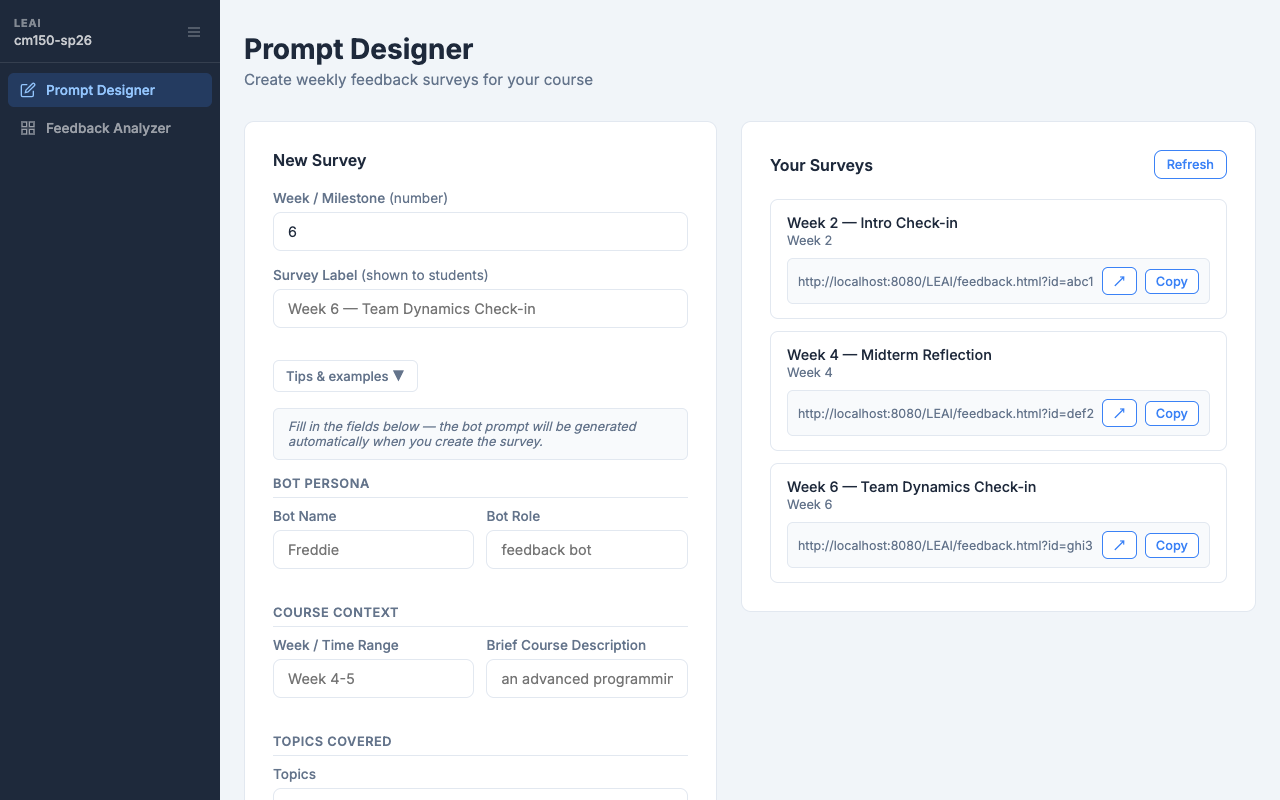
\includegraphics[width=\textwidth]{screenshots/02-prompt-designer-active.png}
\caption{Prompt Designer --- Active Course with Surveys}
\end{figure}

\subsection{Step 3 --- Share the Link}

Your surveys appear on the right panel. Each one has a direct link like:

\begin{center}
\texttt{https://guiilab.github.io/LEAI/feedback.html?id=102}
\end{center}

Click \textbf{Copy} and paste it wherever students will see it --- Canvas announcement, assignment description, or a weekly email. Students don't need to log in; the link takes them directly to the right survey.

\begin{tipbox}
\textbf{One link per survey, per week.} Create a new survey each week with an updated prompt --- don't reuse old links, or responses will mix together in the analyzer.
\end{tipbox}

\section{Part 2: FeedbackCollector (Student View)}

\textbf{What students see when they open the link:}

The page opens directly to a conversation titled with your survey label. The AI sends a welcome message and begins the conversation. Students type freely --- there are no multiple-choice questions.

\begin{figure}[h!]
\centering
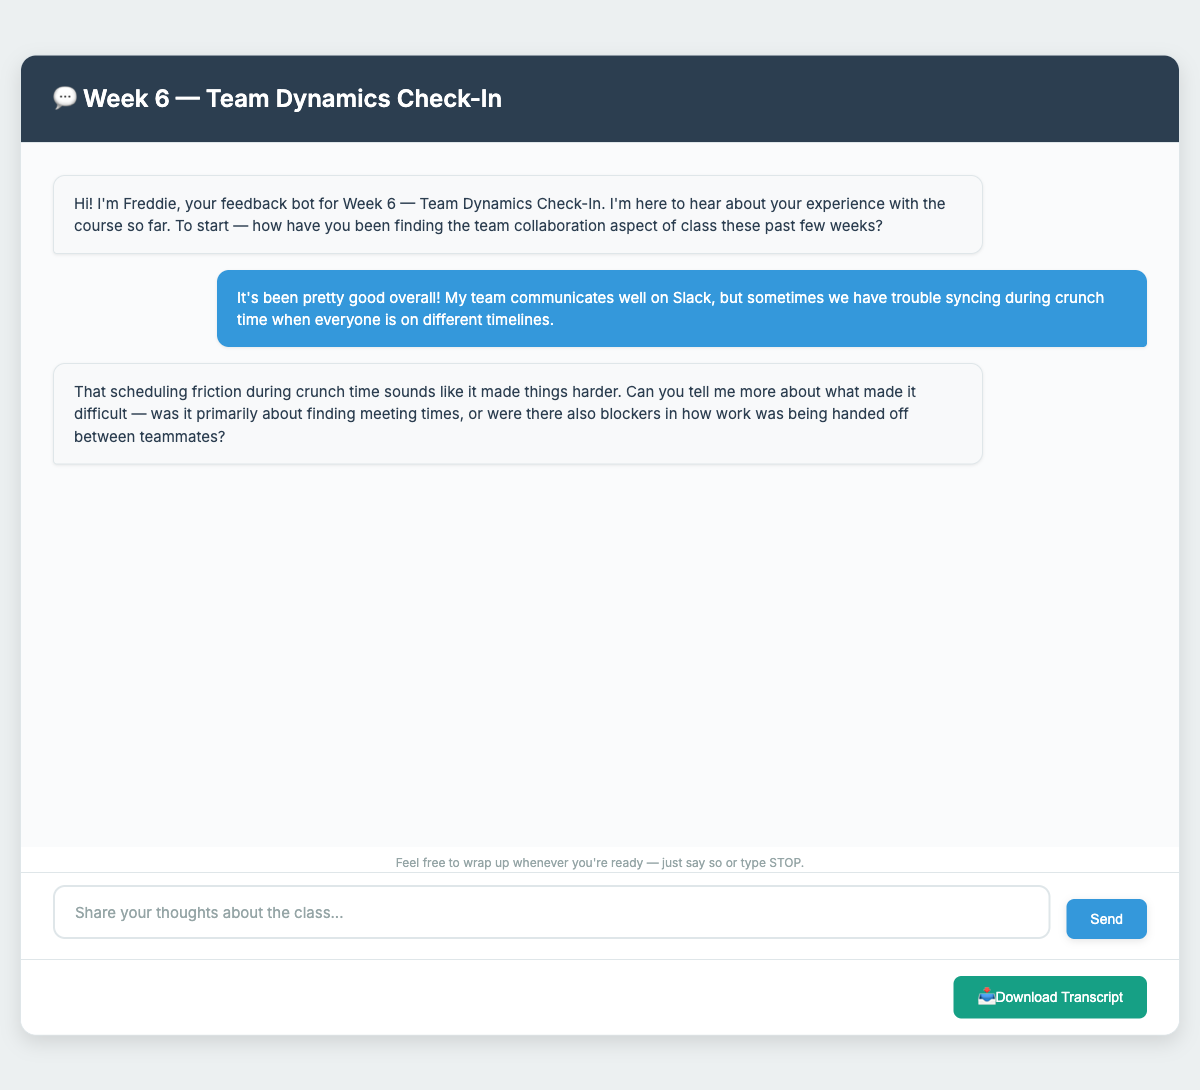
\includegraphics[width=\textwidth]{screenshots/03-feedback-collector-chat.png}
\caption{FeedbackCollector --- Active Conversation}
\end{figure}

\textbf{Key things to communicate to students:}

\begin{itemize}[nosep]
    \item Sessions are \textbf{anonymous} --- no login required, session IDs are randomly generated
    \item A session takes \textbf{5--10 minutes}
    \item Students can \textbf{Download Transcript} at the end if they want a copy
    \item There are no right or wrong answers --- the AI is listening, not grading
\end{itemize}

\textbf{Suggested Canvas announcement text:}

\begin{tipbox}
This week's course check-in is open. It's a short (\textasciitilde5 min) AI conversation --- no login needed, completely anonymous. Your input directly shapes how I adjust the course. Link: [paste link here]
\end{tipbox}

\section{Part 3: Feedback Analyzer}

\textbf{URL:} \url{https://guiilab.github.io/LEAI/FeedbackAnalyzer.html}

This is your read-only dashboard. Enter your Course ID and password to access it.

\begin{figure}[h!]
\centering
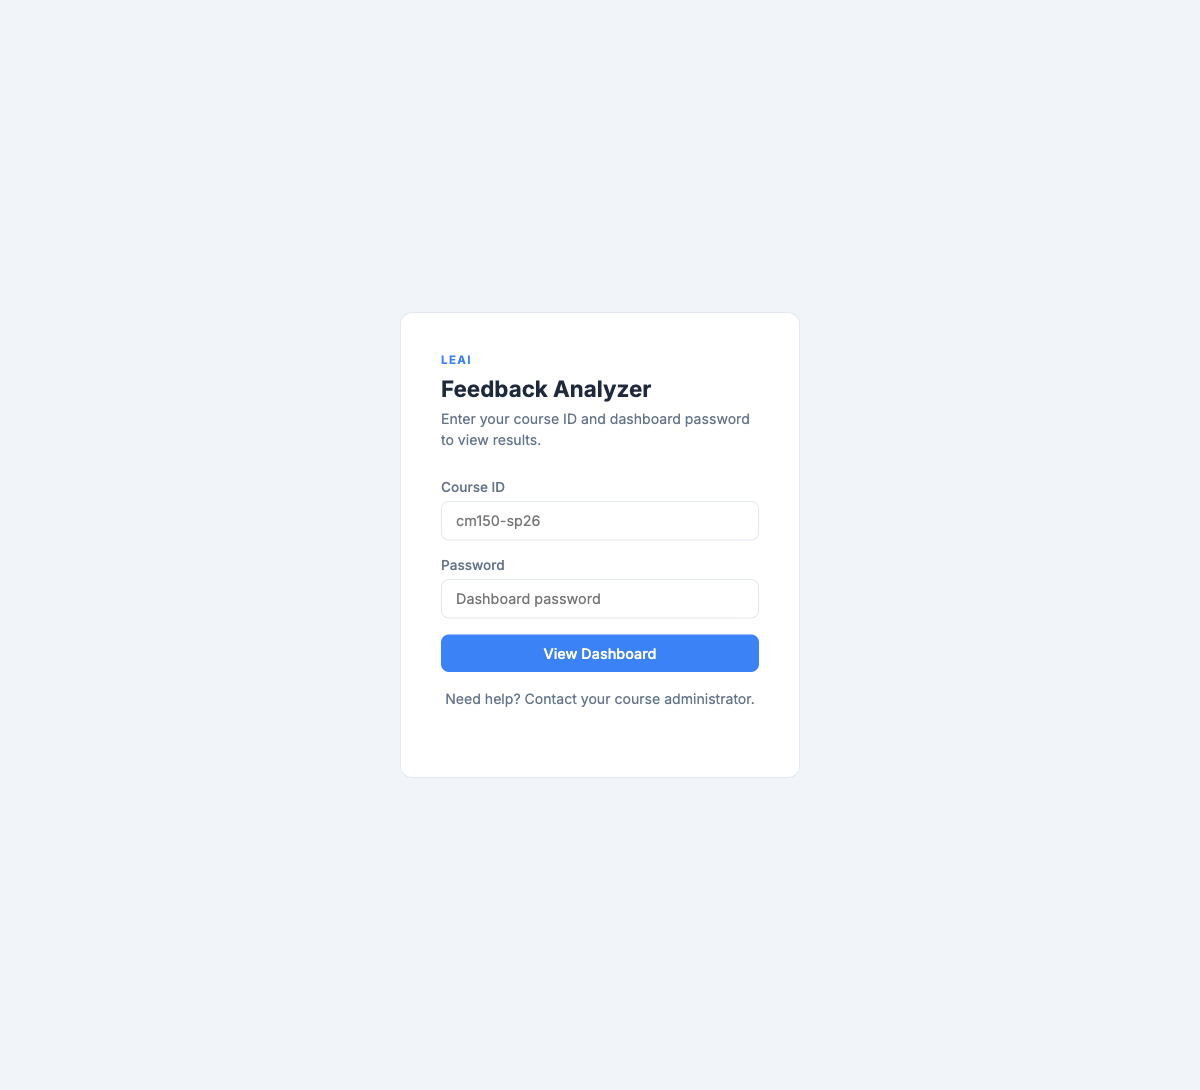
\includegraphics[width=0.7\textwidth]{screenshots/04-analyzer-login.png}
\caption{Feedback Analyzer --- Login}
\end{figure}

\subsection{Course Overview}

After logging in you see all your surveys listed with response counts.

\begin{figure}[h!]
\centering
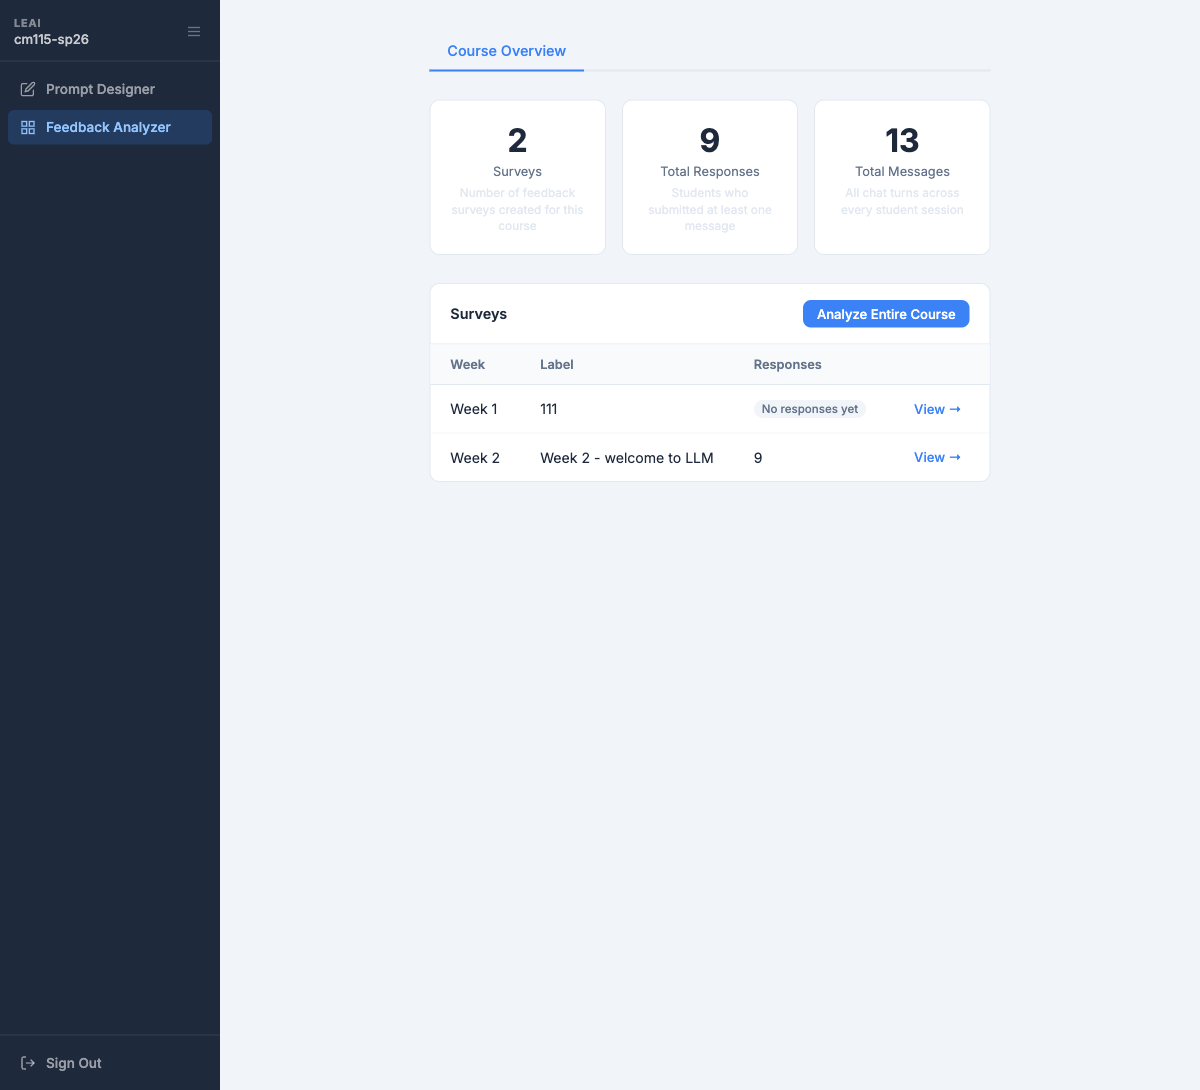
\includegraphics[width=\textwidth]{screenshots/05-analyzer-overview.png}
\caption{Feedback Analyzer --- Course Overview}
\end{figure}

The top stats show total surveys, total responses, and total messages across the whole course. The table below lets you click into any individual survey.

\textbf{Analyze Entire Course} (top right) runs an AI analysis across all surveys --- useful at mid-quarter or end of quarter to see persistent themes.

\subsection{Survey Detail + Analysis}

Click \textbf{View $\rightarrow$} on any survey to open its detail view.

You'll see:
\begin{itemize}[nosep]
    \item \textbf{Responses} --- how many students completed the survey
    \item \textbf{Student Messages} --- total messages sent by students (not AI)
    \item \textbf{Avg.\ Messages / Session} --- a rough proxy for engagement depth
\end{itemize}

Click \textbf{Run Analysis} to generate themes and friction points from that survey's responses.

\begin{figure}[h!]
\centering
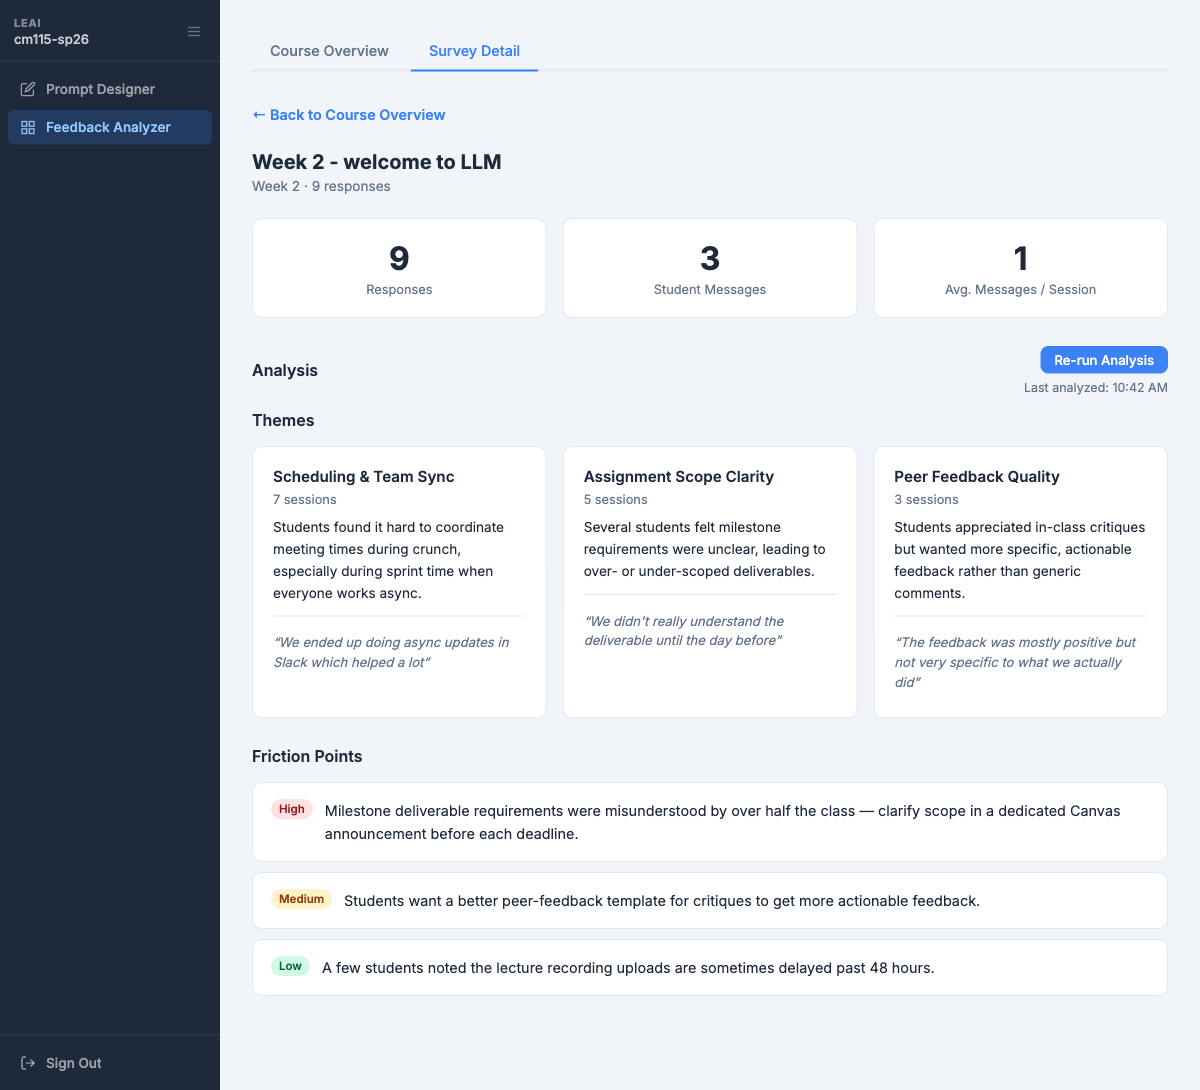
\includegraphics[width=\textwidth]{screenshots/06-analyzer-survey-detail.png}
\caption{Feedback Analyzer --- Survey Analysis}
\end{figure}

\textbf{What the analysis produces:}

\textbf{Theme cards} --- 3--6 recurring topics across student sessions, each with:
\begin{itemize}[nosep]
    \item A label and session count (how many students mentioned it)
    \item A 1--2 sentence summary
    \item 1--2 representative quotes pulled directly from student messages
\end{itemize}

\textbf{Friction Points} --- flagged issues with urgency levels:
\begin{itemize}[nosep]
    \item {\color{urgentred}\textbf{High}} --- address before your next class session
    \item {\color{urgentamber}\textbf{Medium}} --- worth discussing or adjusting soon
    \item {\color{urgentgreen}\textbf{Low}} --- noted but not urgent
\end{itemize}

\begin{tipbox}
\textbf{Minimum for a useful analysis:} aim to collect at least \textbf{8--10 responses} before running analysis. Below that, themes may not be representative. The system will still run, but treat the output as early signal rather than a full report.
\end{tipbox}

\section{Part 4: Importing PDF Reflections}

Some assignments still come in as PDF reflections rather than LEAI chats --- for example, a structured weekly reflection that students upload to Canvas. The Feedback Analyzer has a one-click upload path that reads each PDF, maps its sections to the survey's questions, and lands the responses next to the chat-collected ones --- with a \textbf{PDF} badge so you always know which is which.

\subsection{When to use it}

PDF ingest is available only on \textbf{Structured Reflection} (form-mode) surveys, where each prompt corresponds to a known section in the student's template. The PDF must follow the same section headings as the survey's prompts --- your template's section titles are the matcher, so keep wording consistent across cohorts. Scanned image PDFs (with no embedded text) cannot be read --- re-export from Word or Google Docs as a text PDF.

\subsection{Step 1 --- Open the drawer}

In the Feedback Analyzer, switch to the \textbf{Structured Reflection} tab for the survey you want to add PDFs to, then click \textbf{Upload PDF reflections}. A slide-in drawer opens with a plain-language explainer and a dropzone. The header shows which survey you're uploading into so you can't accidentally land PDFs on the wrong week.

\begin{figure}[H]
\centering
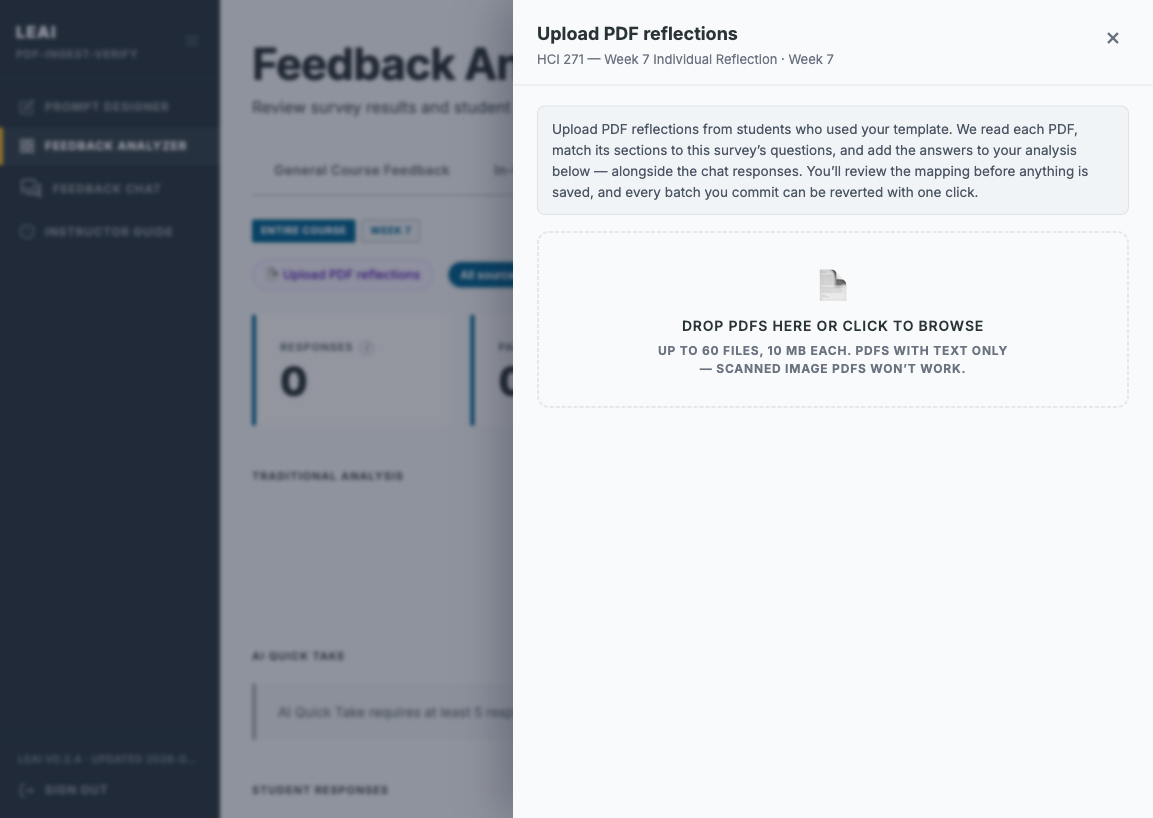
\includegraphics[width=\textwidth]{screenshots/07-pdf-ingest-drawer-open.png}
\caption{Upload drawer --- explainer, dropzone, and survey context in the header}
\end{figure}

\subsection{Step 2 --- Drop the PDFs and confirm student attribution}

Drop in up to 60 PDFs at a time (10 MB each). The system reads each filename and auto-matches it against your course roster --- fuzzy enough to catch \texttt{alice-doe.pdf}, \texttt{doe-alice.pdf}, and \texttt{AliceDoe\_wk7.pdf} all as the same student. Each row shows a small \textit{``Auto-matched from filename --- change if wrong''} hint. If a name is wrong, click the dropdown and pick the correct student.

\begin{figure}[H]
\centering
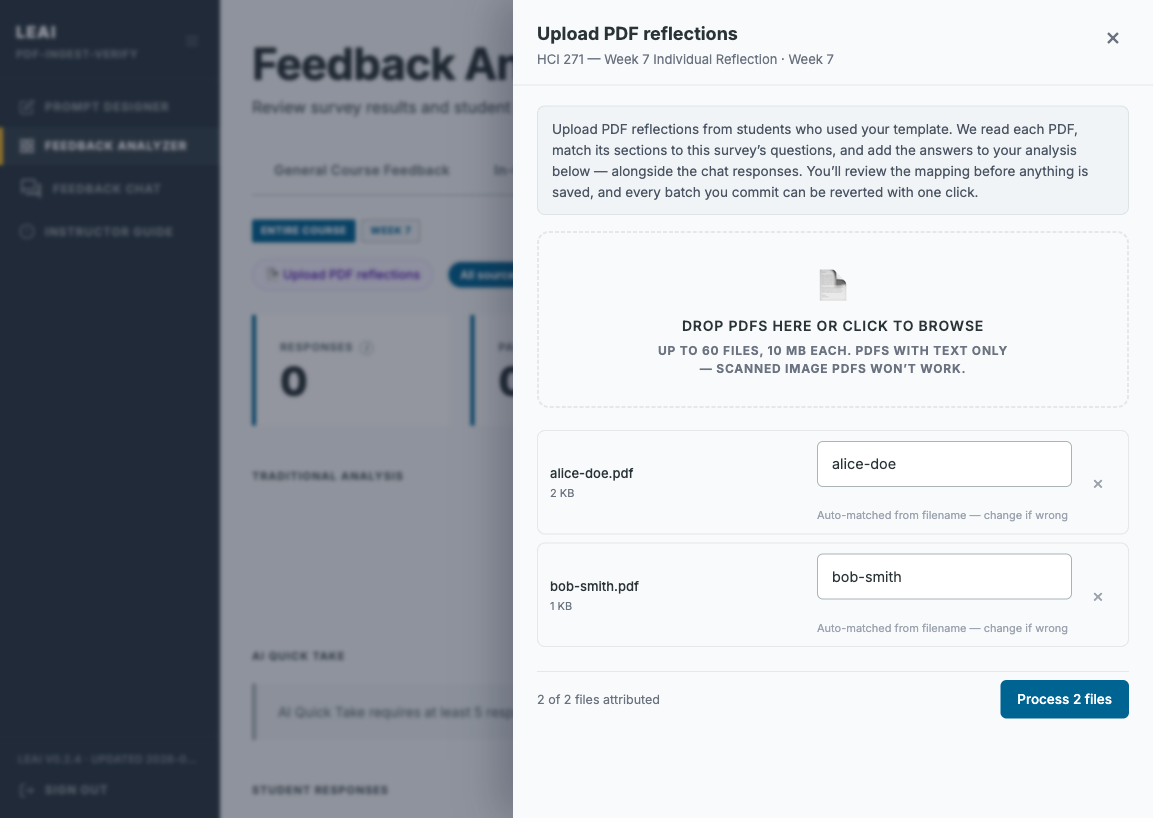
\includegraphics[width=\textwidth]{screenshots/08-pdf-ingest-files-attributed.png}
\caption{Files attributed to roster --- each row auto-matches, with a dropdown for corrections}
\end{figure}

Click \textbf{Process N files}. The server parses each PDF in the background --- the browser tab title becomes \texttt{Reading 0/N PDFs $\cdot$ LEAI} so you can monitor progress from another tab. You can close the drawer and come back; the job keeps running.

\subsection{Step 3 --- Review by exception}

When parsing completes, the drawer flips to a review screen. A banner summarises the result --- e.g.\ ``\textbf{40 PDFs processed} · 36 mapped cleanly · 4 need your attention.''

Only the rows that need work are expanded. PDFs that mapped cleanly are tucked away in a collapsed accordion. For each section the system couldn't auto-detect, you'll see a highlighted ``couldn't find a clear heading'' tag and an empty textarea --- paste the answer in, or leave it blank if the student didn't actually respond.

\begin{figure}[H]
\centering
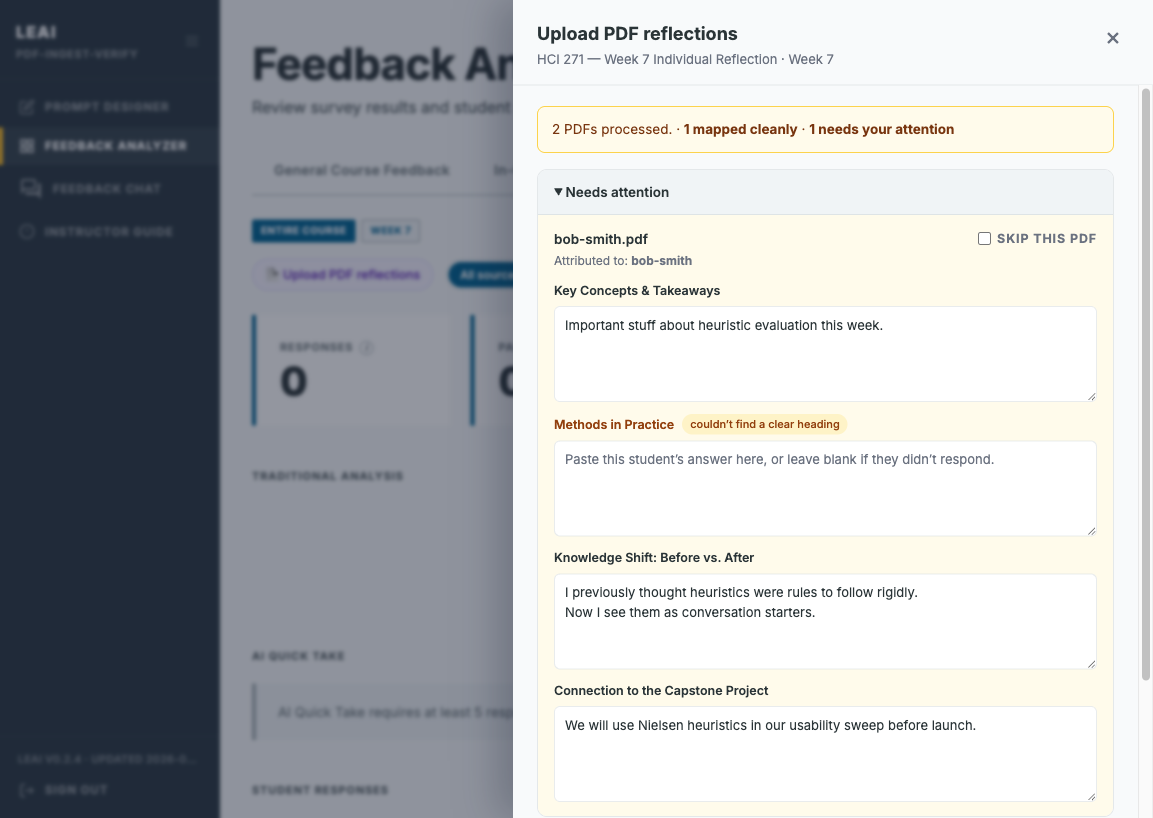
\includegraphics[width=\textwidth]{screenshots/09-pdf-ingest-review-by-exception.png}
\caption{Review by exception --- needs-attention cards expanded, with a missing section highlighted in yellow}
\end{figure}

\textbf{Bulk fill across PDFs.} If the same section is missing from multiple PDFs because of template-wording drift, a yellow bar appears above the Needs Attention group. Paste the corrected answer once and apply it to every empty cell across all affected PDFs. The bulk fill never overwrites a cell that already has content.

\begin{figure}[H]
\centering
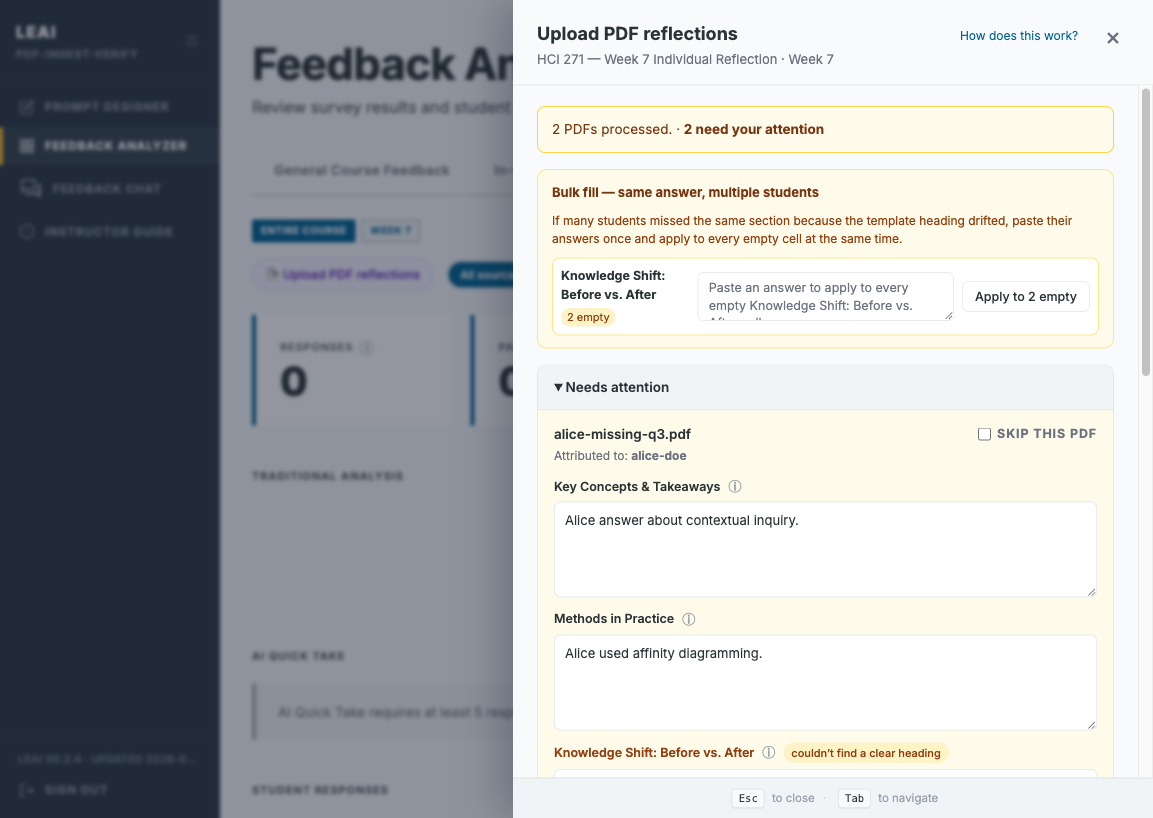
\includegraphics[width=\textwidth]{screenshots/10-pdf-ingest-bulk-fill.png}
\caption{Bulk-fill bar --- paste once, apply to all empty cells in the same prompt}
\end{figure}

\begin{tipbox}
Your edits auto-save as you type. If you close the drawer mid-review, your typed corrections are preserved for up to 7 days and restored when you reopen --- handy if you start review on one device and finish on another.
\end{tipbox}

\subsection{Step 4 --- Commit (with safe defaults for re-uploads)}

When you click \textbf{Commit responses}, you get a final summary: ``About to add \textbf{N} responses from \textbf{M} students.''

If any of those students \emph{already} have a PDF reflection on this survey (for example, you re-uploaded a corrected file), you'll see a per-student dedup choice. The default is always \textbf{Keep existing} --- so a distracted instructor cannot silently overwrite prior data with one click. To overwrite or add a second row, you must explicitly select that option.

\begin{figure}[H]
\centering
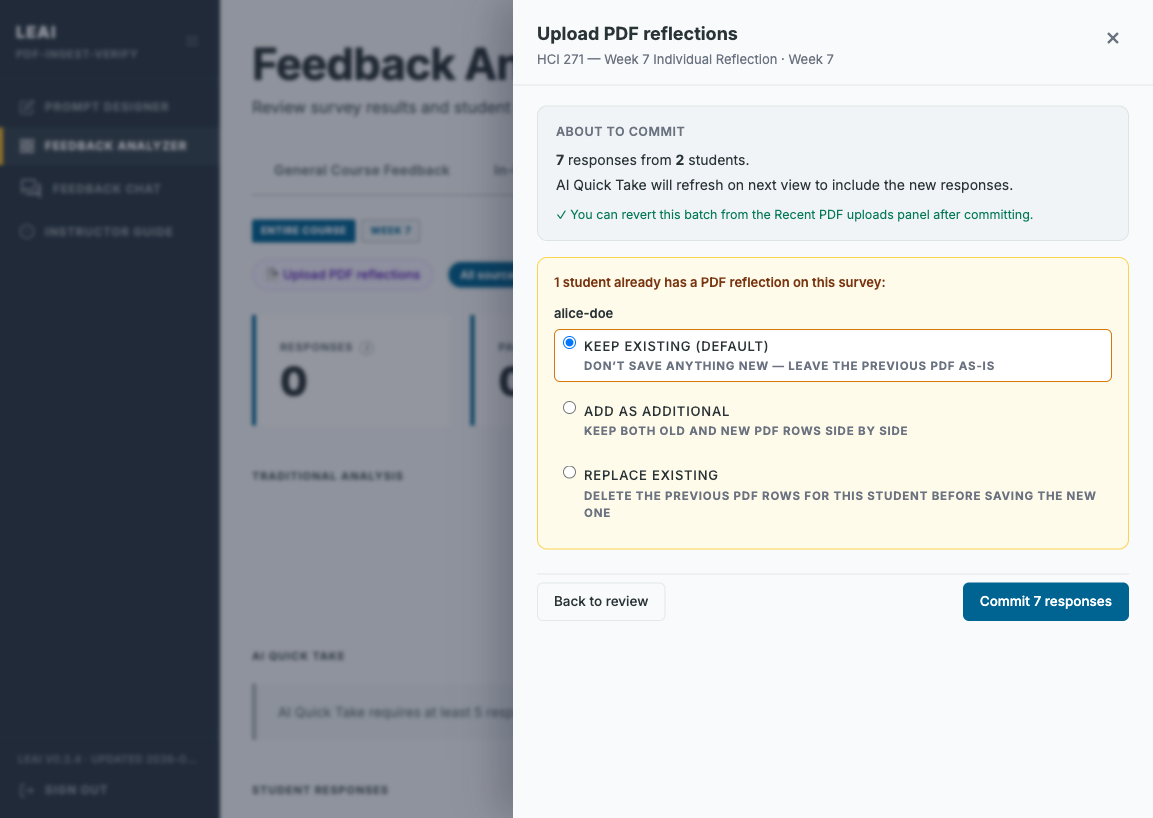
\includegraphics[width=\textwidth]{screenshots/11-pdf-ingest-commit-dedup.png}
\caption{Commit confirmation --- ``Keep existing'' is the default to prevent accidental data loss}
\end{figure}

\subsection{Step 5 --- Done, with a one-click revert if you misclicked}

After commit, a success state confirms how many responses landed and from how many students. The new responses appear immediately in the analyzer below, carrying a \textbf{PDF} badge so you can always tell PDF-derived responses apart from chat ones.

\begin{figure}[H]
\centering
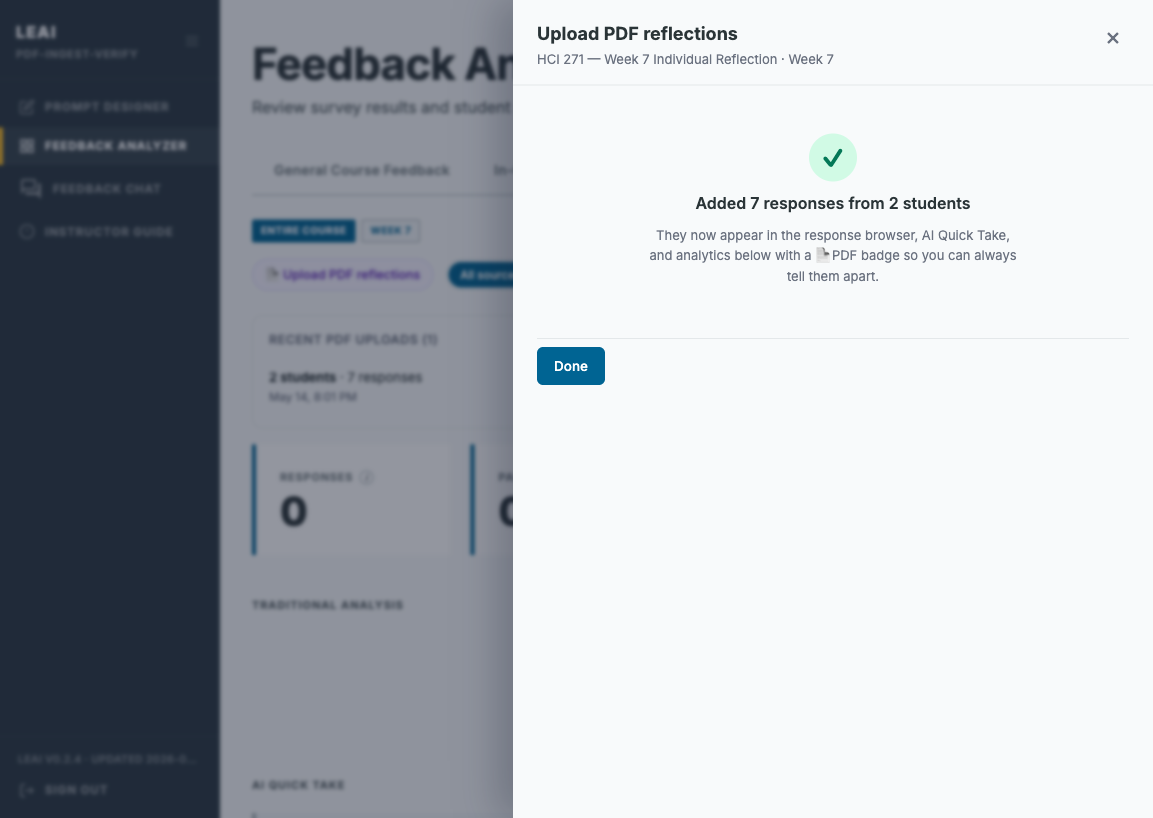
\includegraphics[width=\textwidth]{screenshots/12-pdf-ingest-success.png}
\caption{Success state --- ``Added 7 responses from 2 students''}
\end{figure}

Back in the analyzer, a \textbf{Recent PDF uploads} panel appears above the analytics. Every batch you commit lists there with a one-click \textbf{Revert} button --- so if the wrong batch landed on the wrong week, you can undo the whole thing without touching the database. The AI Quick Take automatically refreshes on next view to include the new responses.

\begin{figure}[H]
\centering
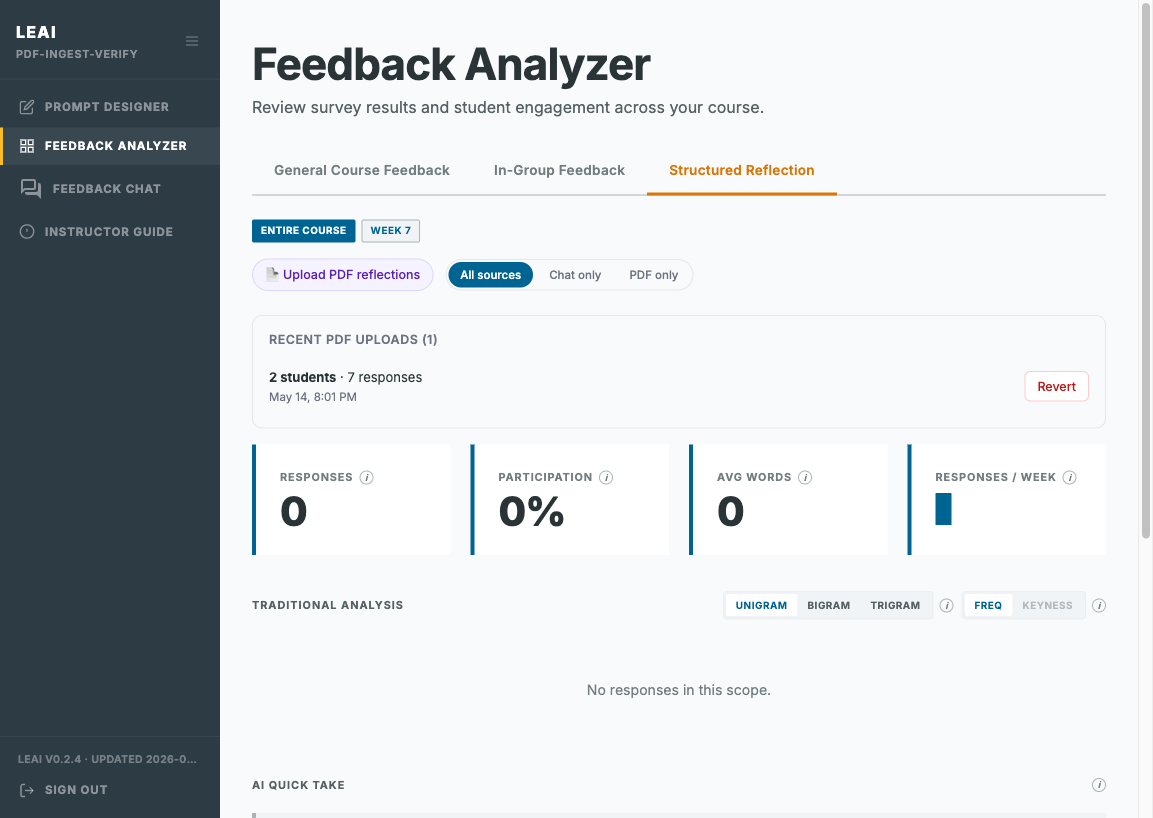
\includegraphics[width=\textwidth]{screenshots/13-pdf-ingest-after-commit.png}
\caption{Analyzer after commit --- Recent PDF uploads panel with one-click Revert per batch}
\end{figure}

\subsection{Safety summary}

\begin{itemize}[nosep]
    \item \textbf{Nothing destructive without your explicit choice.} ``Replace existing'' is never the default --- you have to pick it.
    \item \textbf{Every batch is revertable.} Until you delete the manifest row, any commit can be undone in one click.
    \item \textbf{Edits auto-save.} Mid-review corrections persist for up to 7 days across drawer closes.
    \item \textbf{Original PDFs are never stored.} The server extracts the text and discards the binary; only per-student, per-prompt answers live in the database.
\end{itemize}

\subsection{Limits \& gotchas}

\begin{itemize}[nosep]
    \item Scanned image PDFs (no embedded text) cannot be read --- re-export as a text-based PDF.
    \item Password-protected PDFs are rejected.
    \item One PDF over 10 MB, or a batch over 50 MB, is refused --- split into smaller batches.
    \item In General or In-Group survey modes, PDF ingest is unavailable; switch the survey to Structured Reflection mode if that's the right shape for it.
\end{itemize}

\FloatBarrier  % flush all PDF-ingest figures before next section

\section{Weekly Workflow (5 min/week)}

\begin{table}[h!]
\centering
\begin{tabular}{@{}lp{10cm}@{}}
\toprule
\textbf{Day} & \textbf{Action} \\
\midrule
Monday & Create a new survey in Prompt Designer, copy the link. Post link to Canvas with a brief note. \\
Wednesday & Check response count in Feedback Analyzer (aim for 50\%+ of class). \\
Thursday & Run Analysis --- read themes before Friday's class. Adjust pacing, address friction points, or clarify assignments. \\
Friday & Optional: briefly acknowledge patterns in class. (``Several of you mentioned confusion about milestone scope --- let me clarify\ldots'') \\
\bottomrule
\end{tabular}
\end{table}

\section{FAQ}

\textbf{Can I have multiple courses?}\\
Yes --- each course has its own Course ID and password. Create separate courses for each section.

\textbf{Can my TA access the dashboard?}\\
Yes --- share your Course ID and dashboard password with them. There's no separate TA login.

\textbf{Do students need a UCSC login?}\\
No. The link works for anyone. Students don't create accounts.

\textbf{Can I edit a survey after creating it?}\\
Not currently. If you need to change the prompt, create a new survey and share the new link. Old responses stay attached to the original survey.

\textbf{How many surveys should I run per quarter?}\\
3--4 is a reasonable target --- week 3, 6, 9, and optionally week 1 (orientation) or post-milestone. More is fine, but student fatigue is real past \textasciitilde4 per quarter.

\textbf{What if analysis returns something unexpected?}\\
The AI analysis is a starting point, not a verdict. Read a few raw sessions in the session list if something seems off. Final instructional decisions are always yours.

\section{Getting Help}

Contact Jiahong Li (\href{mailto:jli906@ucsc.edu}{jli906@ucsc.edu}) for technical issues, feature requests, or onboarding support.

\end{document}
